% --------------------------------------------------------------
% This is all preamble stuff that you don't have to worry about.
% Head down to where it says "Start here"
% --------------------------------------------------------------
 
\documentclass[12pt]{article}
 
\usepackage[margin=1in]{geometry} 
\usepackage{amsmath,amsthm,amssymb}
\usepackage{braket}
\usepackage{graphicx}
\usepackage{calligra}
\usepackage{calrsfs}
\usepackage{subcaption}
\usepackage{listings}
\newcommand{\N}{\mathbb{N}}
\newcommand{\Z}{\mathbb{Z}}
 
\newenvironment{theorem}[2][Theorem]{\begin{trivlist}
\item[\hskip \labelsep {\bfseries #1}\hskip \labelsep {\bfseries #2.}]}{\end{trivlist}}
\newenvironment{lemma}[2][Lemma]{\begin{trivlist}
\item[\hskip \labelsep {\bfseries #1}\hskip \labelsep {\bfseries #2.}]}{\end{trivlist}}
\newenvironment{exercise}[2][Exercise]{\begin{trivlist}
\item[\hskip \labelsep {\bfseries #1}\hskip \labelsep {\bfseries #2.}]}{\end{trivlist}}
\newenvironment{reflection}[2][Reflection]{\begin{trivlist}
\item[\hskip \labelsep {\bfseries #1}\hskip \labelsep {\bfseries #2.}]}{\end{trivlist}}
\newenvironment{proposition}[2][Proposition]{\begin{trivlist}
\item[\hskip \labelsep {\bfseries #1}\hskip \labelsep {\bfseries #2.}]}{\end{trivlist}}
\newenvironment{corollary}[2][Corollary]{\begin{trivlist}
\item[\hskip \labelsep {\bfseries #1}\hskip \labelsep {\bfseries #2.}]}{\end{trivlist}}
 
\begin{document}
 
% --------------------------------------------------------------
%                         Start here
% --------------------------------------------------------------
 
%\renewcommand{\qedsymbol}{\filledbox}
 
\title{HW5}
\author{Carl Mueller\\ %replace with your name
CSCI 5254 - Convex Optimization} %if necessary, replace with your course title
\maketitle

\subsection*{6.1}
\begin{proposition}{1}
\begin{align}
log(x+1) \le x\\ -log(x+1) \ge x\\ x > -1
\end{align}
\end{proposition}

\begin{proposition}{2}
\begin{align}
-log(1-x)\ \text{is convex}
\end{align}
\end{proposition}
\begin{proposition}{3}
\begin{align}
\phi(||u||_{\infty}) = -a^2log(1-\frac{||u||_{\infty}}{a^2})
\end{align}
\end{proposition}

Left inequality working backwards:
\begin{equation*}
\begin{aligned}
||u||_{2}^{2} \le -a^2\sum_{i=1}^{m}log(1 - \frac{u_{i}^{2}}{a^2})\\
\sum_{i=1}^{m}\frac{|u_i|^2}{a^2} \le -\sum_{i=1}^{m}log(1 - \frac{u_{i}^{2}}{a^2})\\
\end{aligned}
\end{equation*}
Given proposition 1:
\begin{equation*}
\begin{aligned}
\sum_{i=1}^{m}\frac{|u_i|^2}{a^2} \le -\sum_{i=1}^{m}log(1 - \frac{u_{i}^{2}}{a^2})\\
\text{true when: }\\
- \frac{u_{i}^{2}}{a^2} \ge -1
\end{aligned}
\end{equation*}

Right inequality:
\begin{equation*}
\begin{aligned}
\text{Given: } u_{i}^{2} \le ||u_i||_{\infty}^{2}\\
\sum_{i=1}^{m}-log(1 - \frac{u_{i}^{2}}{a^2}) \le \sum_{i=1}^{m}-log(1 - \frac{||u_{i}||_{\infty}^{2}}{a^2})\ \text{given proposition 1}\\
\sum_{i=1}^{m}-log(1 - \frac{u_{i}^{2}}{a^2}) \le \frac{u_{i}^{2}}{||u||_{2}^{\infty}}\sum_{i=1}^{m}-log(1 - \frac{||u_{i}||_{\infty}^{2}}{a^2})\ \text{given $\frac{u_{i}^{2}}{||u||_{2}^{\infty}} \ge 1$}\\
-a^2\sum_{i=1}^{m}log(1 - \frac{u_{i}^{2}}{a^2}) \le -a^2\frac{u_{i}^{2}}{||u||_{2}^{\infty}}\sum_{i=1}^{m}log(1 - \frac{||u_{i}||_{\infty}^{2}}{a^2})\\
-a^2\sum_{i=1}^{m}log(1 - \frac{u_{i}^{2}}{a^2}) \le \frac{u_{i}^{2}}{||u||_{2}^{\infty}}\phi(||u||_{\infty})\\
\end{aligned}
\end{equation*}

\subsection*{6.9}
To show convexity, the following level set must be convex:

$$S_{\alpha} = \set{t_i| \max_{i=1,\dots,k}|\frac{p(t_i)}{q(t_i)} - y_i| \le \alpha}$$

Due to absolute value, following inequalities must hold:
\begin{equation*}
\begin{aligned}
-\alpha q(t_i) \le y_i q(t_i)-p(t_i) \le \alpha q(t_i)
\end{aligned}
\end{equation*}
 This is represent two inequalities that define a polyhedron and is therefore convex. Since the level set is convex,
 the original minimzation problem is at least quasiconvex.

\subsection*{7.3}

\begin{proposition}{1}
\begin{align}
P(x|y=1) = \frac{1}{\sqrt{2 \pi}}\int_{x}^{\infty}e^{\frac{-z^2}{2}}dz\\
P(x|y=0) = 1 - \frac{1}{\sqrt{2 \pi}}\int_{x}^{\infty}e^{\frac{-z^2}{2}}dz
\end{align}
\end{proposition}

Ordering probability terms in order of $y=1$ and $y=0$, our total probability is:
\begin{equation*}
\begin{aligned}
p(a,b) = \prod_{i=1}^{q}P_i(a^Tu_i+b|y=1)\prod_{i=q+1}^{m}(1-P_i(a^Tu_i+b|y=0))\\
\end{aligned}
\end{equation*}
The negative log likelihood:
\begin{equation*}
\begin{aligned}
l(a,b) = \sum_{i=1}^{q}-log(P_i(a^Tu_i+b|y=1))+\sum_{i=q+1}^{m}-log(1-P_i(a^Tu_i+b|y=0))
\end{aligned}
\end{equation*}
The negative log likelihood is a convex function, so minimizing this function is a convex optimization problem.

\subsection*{7.4}
\subsubsection*{a)}
\begin{proposition}{1}
\begin{align}
\text{Sample mean: }
u = \frac{1}{N}\sum_{k=1}^{N}y_k\\
\text{Covariance: }
Y = \frac{1}{N}\sum_{k=1}^{N}(y_k-u)(y_k-u)^T
\end{align}
\end{proposition}

\begin{equation*}
\begin{aligned}
-\frac{N}{2}nlog(2\pi)-\frac{N}{2}log(det(R))- \frac{1}{2}R^{-1}\sum_{k=1}^{N}(y_k-a)(y_k-a)^T\\
= -\frac{N}{2}nlog(2\pi)-\frac{N}{2}log(det(R))- \frac{1}{2}R^{-1}\sum_{k=1}^{N}(y_ky_k^T-ay_k^T-y_ka^T+aa^T)\\
= -\frac{N}{2}nlog(2\pi)-\frac{N}{2}log(det(R))- \frac{1}{2}R^{-1}(\sum_{k=1}^{N}y_ky_k^T-\sum_{k=1}^{N}ay_k^T-\sum_{k=1}^{N}y_ka^T+\sum_{k=1}^{N}aa^T))\\
= -\frac{N}{2}nlog(2\pi)-\frac{N}{2}log(det(R))- \frac{1}{2}R^{-1}(\sum_{k=1}^{N}y_ky_k^T-\sum_{k=1}^{N}ay_k^T-\sum_{k=1}^{N}y_ka^T+Naa^T)\\
\end{aligned}
\end{equation*}

Substitute sample mean:
\begin{equation*}
\begin{aligned}
= -\frac{N}{2}nlog(2\pi)-\frac{N}{2}log(det(R))- \frac{1}{2}R^{-1}\sum_{k=1}^{N}y_ky_k^T-Nay^T-Nua^T+Naa^T\\
= R^{-1}\sum_{k=1}^{N}(y_k-a)(y_k-a)^T-R^{-1}N(a-u)(a-u)^T\\
= -\frac{N}{2}nlog(2\pi)-\frac{N}{2}log(det(R))- \frac{1}{2}(NR^{-1}Y + R^{-1}N(a-u)(a-u)^T)\\
= -\frac{N}{2}nlog(2\pi)-\frac{N}{2}log(det(R))- \frac{1}{2}(Ntr(R^{-1}Y) + N(a-u)R^{-1}(a-u)^T)
\end{aligned}
\end{equation*}

Set the gradient to zero to see $a$ and $R$ optimal values.
\begin{equation*}
\begin{aligned}
\nabla_a l(R,a) = -2R^{-1}(a-u) = 0\\
\therefore a=u \\
\nabla_R l(R,a) = -R^{-1} + R^{-1}(Y - (a-u)(a-u)^T)R^{-1} = 0\\
R = Y + (a-u)(a-u)^T\\
R = Y + (0)(0)^T\\
\therefore R=Y
\end{aligned}
\end{equation*}

\subsection*{7.8}

Express sign function as a probability where we order values with $y>1$ followed by $y<0$:
\begin{equation*}
\begin{aligned}
\prod_{i=1}^{k}prob(a_i^Tx + b_i + v_i > 0)\prod_{i=k+1}^{m}prob(a_i^Tx + b_i + v_i < 0)
\end{aligned}
\end{equation*}

Since $a_i$ and $b_i$ are known values, the only RV is the noise term. We can epxress $v_i$ as an expression of $a_i^Tx+b_i$. P represents the cumulative density function of $v_i$. We can represent the probability as follows:
\begin{equation*}
\begin{aligned}
\prod_{i=1}^{k}P(-a_i^Tx-b_i)\prod_{i=k+1}^{m}1-P(-a_i^Tx-b_i) 
\end{aligned}
\end{equation*}

Log likelihood below is concave so if we maximize, we obtain a convex problem:
\begin{equation*}
\begin{aligned}
l(x) = \sum_{i=1}^{k}log(P(-a_i^Tx-b_i))+\sum_{i=k+1}^{m}log(1-P(-a_i^Tx-b_i))\\ 
\end{aligned}
\end{equation*}

\subsection*{7.9}
Given $$y_i = f(a_i^Tx +b_i +v_i), i=1,\dots,m$$
We know that $a_i$ and $b_i$ are knowns, so lets expression the random variable $v_i$ as an expression of all other terms. We assume that $f$ is an invertible function.
$$v_i = f^{-1}(y_i)-a_i^Tx-b_i$$
The probability of observing $y_i,\dots,y_m$ is:
\begin{equation*}
\begin{aligned}
\prod_{i=1}^{m}prob(f^{-1}(y_i)-a_i^Tx-b_i)\\
l(x, f) = \sum_{i=1}^{m}log(prob(f^{-1}(y_i)-a_i^Tx-b_i))
\end{aligned}
\end{equation*}
This log probability is concave w.r.t x and f. Thus maximizing generates a convex optimization problem.\\\\

\textbf{Additional Exercises:}\\\\
\subsection*{3.9}
\subsubsection*{a)}
Given: $$z = [\Re x, \Im x]$$

Setup a system of equations using the vector breakdown of x for its $\Re$ and $\Im$ components:
\begin{equation*}
\begin{aligned}
||x||_2^2 = ||z||_2^2\\
\begin{bmatrix}
\Re A & -\Im A\\
\Im A & \Re A
\end{bmatrix}
\begin{bmatrix}
\Re x \\
\Im x
\end{bmatrix}=
\begin{bmatrix}
\Re b\\
\Im b
\end{bmatrix}
\end{aligned}
\end{equation*}

This becomes the optimization problem:
\begin{equation*}
\begin{aligned}
& \underset{z}{\text{minimize}}
& & ||z||_2\\
& \text{subject to}\
& &
\begin{bmatrix}
\Re A & -\Im A\\
\Im A & \Re A
\end{bmatrix}
\begin{bmatrix}
\Re x \\
\Im x
\end{bmatrix}=
\begin{bmatrix}
\Re b\\
\Im b
\end{bmatrix}
\end{aligned}
\end{equation*}

\subsubsection*{b)}
Define the second order cone:
\begin{equation*}
\begin{aligned}
K_i = \set{(z,t)| ||z||_2 \le t}
\end{aligned}
\end{equation*}
The SOCP:
\begin{equation*}
\begin{aligned}
& \underset{}{\text{minimize}}
& & t\\
& \text{subject to}\
& |z||_2\\
& &
\begin{bmatrix}
\Re A & -\Im A\\
\Im A & \Re A
\end{bmatrix}
\begin{bmatrix}
\Re x \\
\Im x
\end{bmatrix}=
\begin{bmatrix}
\Re b\\
\Im b
\end{bmatrix}\end{aligned}
\end{equation*}
\subsubsection*{c)}
\textbf{Code:}
\begin{lstlisting}
randn('state',0);
m = 30; n = 100;
Are = randn(m,n); Aim = randn(m,n);
bre = randn(m,1); bim = randn(m,1);
A = Are + i*Aim;
b = bre + i*bim;

Atot = [Are -Aim; Aim Are];
btot = [bre; bim];
z_2 = Atot'*inv(Atot*Atot')*btot;
x_2 = z_2(1:100) + i*z_2(101:200);

cvx_begin
    variable x(n) complex
    minimize( norm(x) )
    subject to
    A*x == b;
cvx_end

cvx_begin
    variable xinf(n) complex
    minimize( norm(xinf,Inf) )
    subject to
    A*xinf == b;
cvx_end

figure(1)
scatter(real(x),imag(x)), hold on,
scatter(real(xinf),imag(xinf),[],'filled'), hold off,
axis([-0.2 0.2 -0.2 0.2]), axis square,
xlabel('Re x'); ylabel('Im x');
\end{lstlisting}
Results:
\begin{figure}[h]
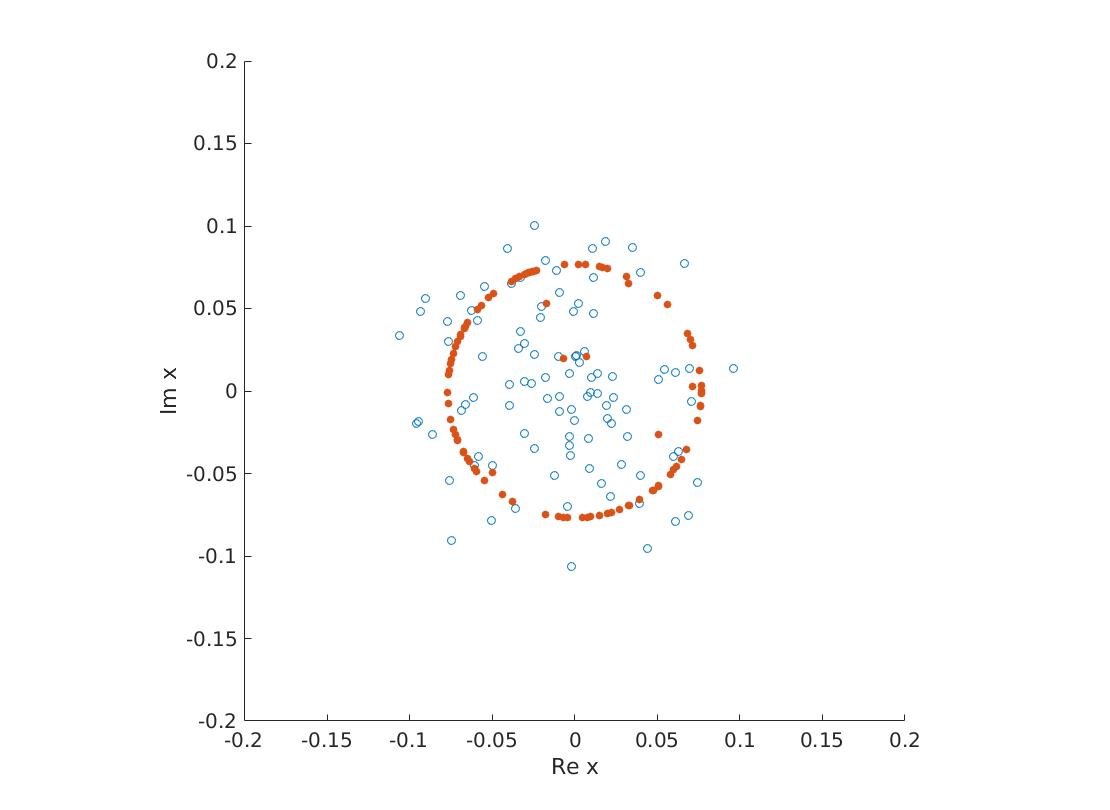
\includegraphics[scale=.25]{39c.jpg}
\end{figure}
The red dots represent the infinity norm.

\subsection*{4.1}
\subsubsection*{a)}
Code:
\begin{lstlisting}
M = [1 -1/2; -1/2 2];
m = [-1 0]';
A = [1 2; 1 -4; 5 76];
b = [-2 -3 1]';
delta = .1

cvx_begin
    variable x(2)
    dual variable y
    minimize(quad_form(x, M)+m'*x)
    subject to
        y: A*x <= b;
cvx_end
p_star = cvx_optval
y
x
\end{lstlisting}
\textbf{Results:}\\
p\_star = 8.2222\\
y = \\1.8994\\
    3.4684\\
    0.0931\\
x =\\-2.3333\\
    0.1667\\\\
\underline{KKT Conditions}\\
Primal:\\
$$x_1^* + 2x_2^* \le u_1$$
$$x_1^* + -4x_2^* \le u_2$$
$$5x_1^* + 76x_2^*\le 1$$
Dual:\\
$$\lambda_1^*, \lambda_2^*, \lambda_3^* \ge 0$$
Complementary Slackness:
$$\lambda_1^*(x_1^* + 2x_2^* - u_1)=0$$
$$\lambda_2^*(x_1^* + -4x_2^* - u_2)=0$$
$$\lambda_3^*(5x_1^* + 76x_2^* - 1)=0$$
First Order Conditions:
$$4x_2^*-x_1^*+2\lambda_1^*-4\lambda_2^*+76\lambda_3^*=0$$
$$2x_1^* -x_2^*-1+\lambda_1^*+\lambda_2^*+5\lambda_2^*=0$$
\subsubsection*{b)}
\textbf{Code:}
\begin{lstlisting}
M = [1 -1/2; -1/2 2];
m = [-1 0]';
A = [1 2; 1 -4; 5 76];
b = [-2 -3 1]';

cvx_begin
    variable x(2)
    dual variable y
    minimize(quad_form(x, M)+m'*x)
    subject to
        y: A*x <= b;
cvx_end
p_star = cvx_optval

array = [0 -1 1];
table = [];
delta = 0.1;

for i = array
    for j = array
        p_pred = p_star - [y(1) y(2)]*[i; j]*delta;
        cvx_begin
            variable x(2)
            minimize(quad_form(x,M)+m'*x)
            subject to
                A*x <= b+[i;j;0]*delta
        cvx_end
        p_exact = cvx_optval;
        table = [table; i*delta j*delta p_pred p_exact]
    end
end
\end{lstlisting}
\textbf{Results:}
\begin{center}
  \begin{tabular}{ | c | c | c | c |}
  \hline
    $d_1$ & $d_2$ & $p^*_{pred}$ & $p^*_{exact}$ \\ \hline
    0 &        0  &  8.2222  &  8.2222 \\ \hline
    0&   -0.1000    &8.5691   & 8.7064 \\ \hline
    0    &0.1000    &7.8754    &7.9800 \\ \hline
    -0.1000&         0 &   8.4122 &    8.5650 \\ \hline
    -0.1000&   -0.1000  &  8.7590  &  8.8156 \\ \hline
    -0.1000&    0.1000  &  8.0653  &  8.3189 \\ \hline
    0.1000 &        0   & 8.0323   & 8.2222 \\ \hline
    0.1000 &  -0.1000    & 8.3791   & 8.7064 \\ \hline
    0.1000 &   0.1000   & 7.6854   & 7.7515 \\ \hline
  \end{tabular}
\end{center}
We can see that $p^*_{pred} \le p^*_{exact}$ for all pertubations.

\subsection*{5.2}
The objective function $\underset{i=1,\dots,k}{\max}|f(t_i)-y_i|$ is not convex, however it is quasiconvex: $$\set{t,y,\alpha | \underset{i=1,\dots,k}{\max}|f(t_i)-y_i| \le \alpha}$$
as it is a linear inequality.\\\\

\begin{figure}[h]
\centering
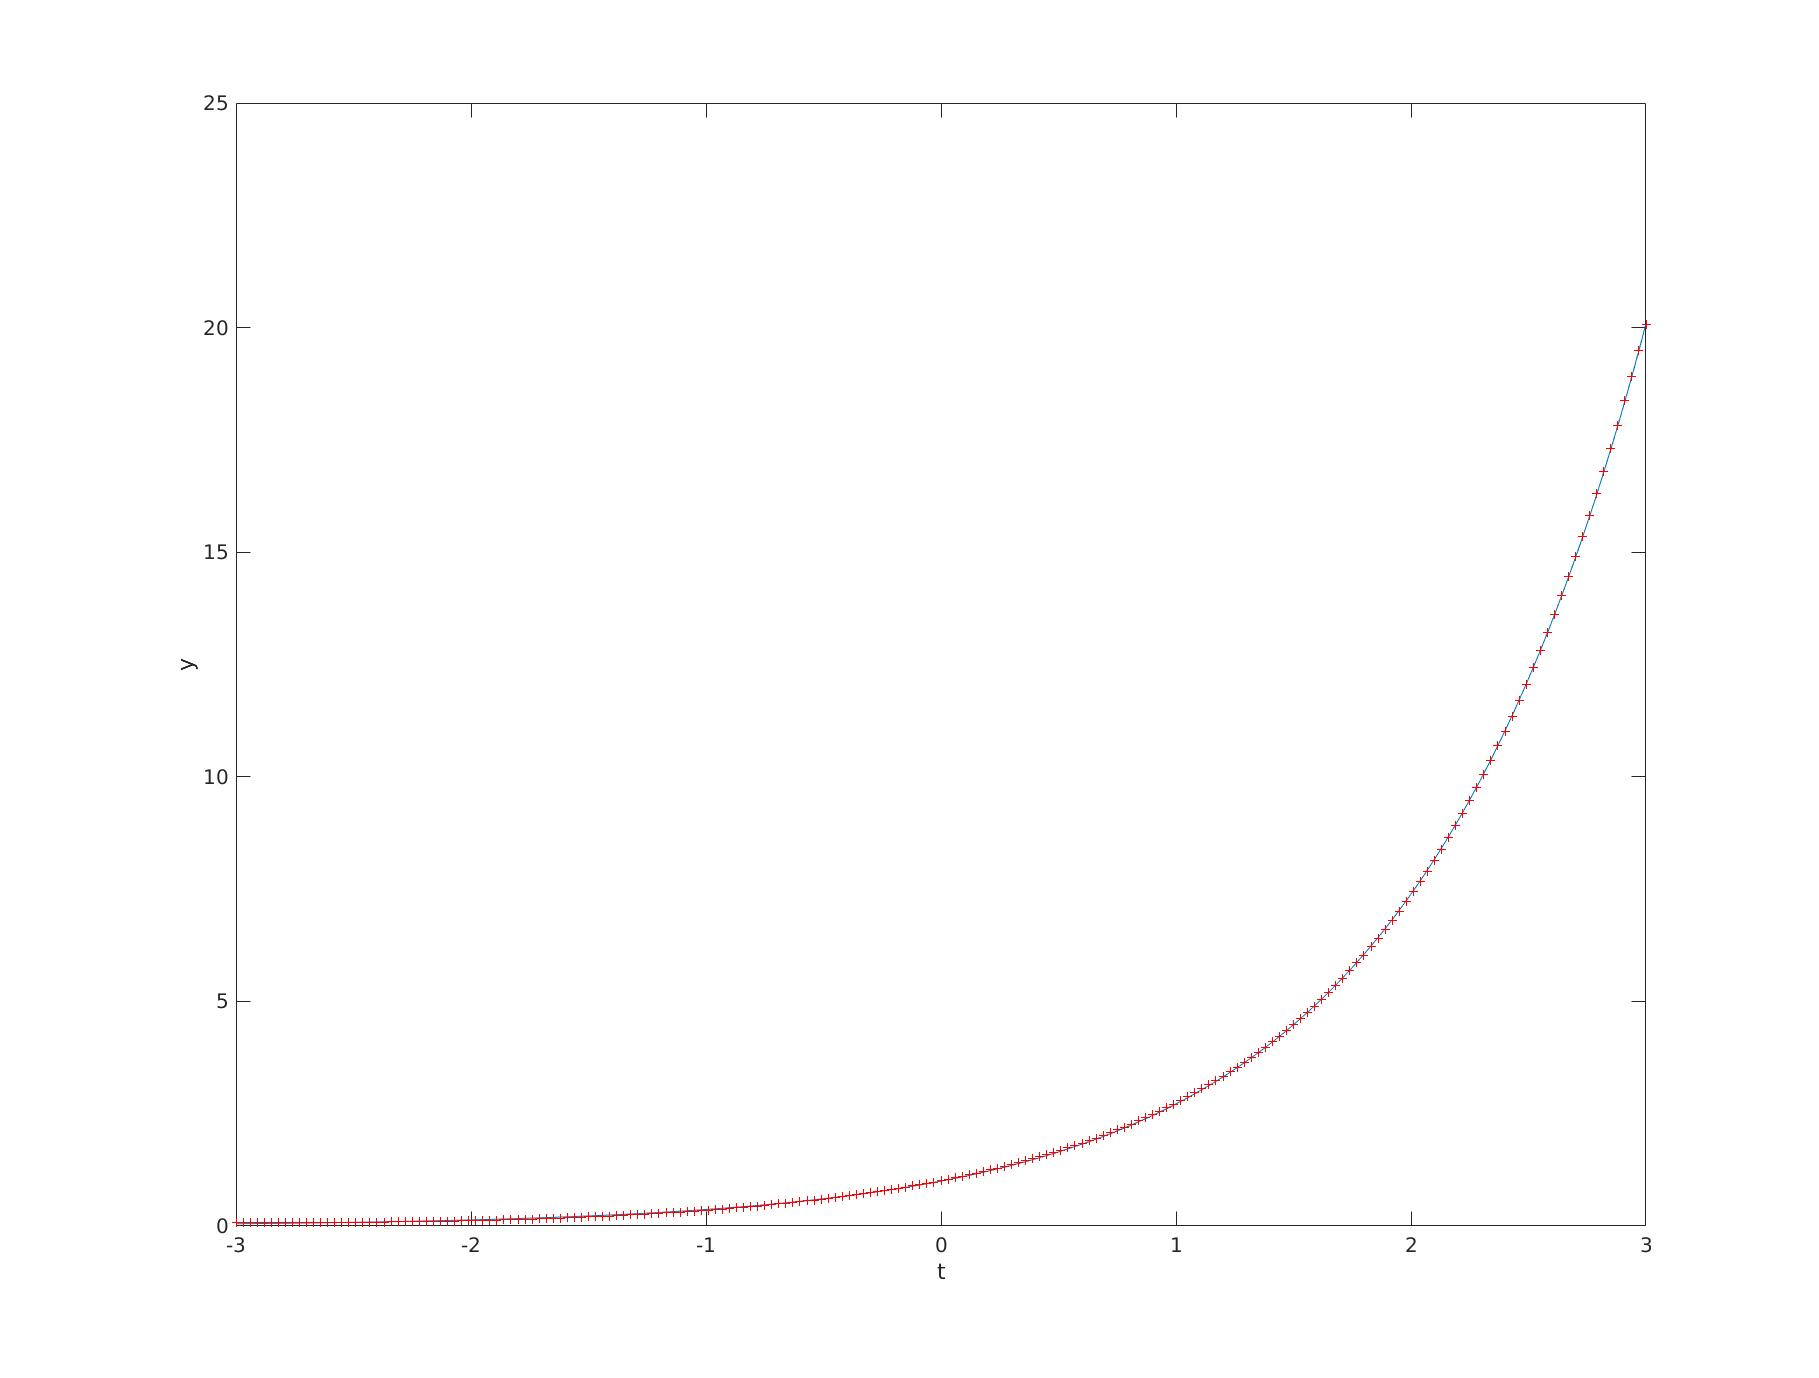
\includegraphics[scale=.2]{52_1.jpg}
\caption{Data and optimal function fit.}
\end{figure}
\begin{figure}[h]
\centering
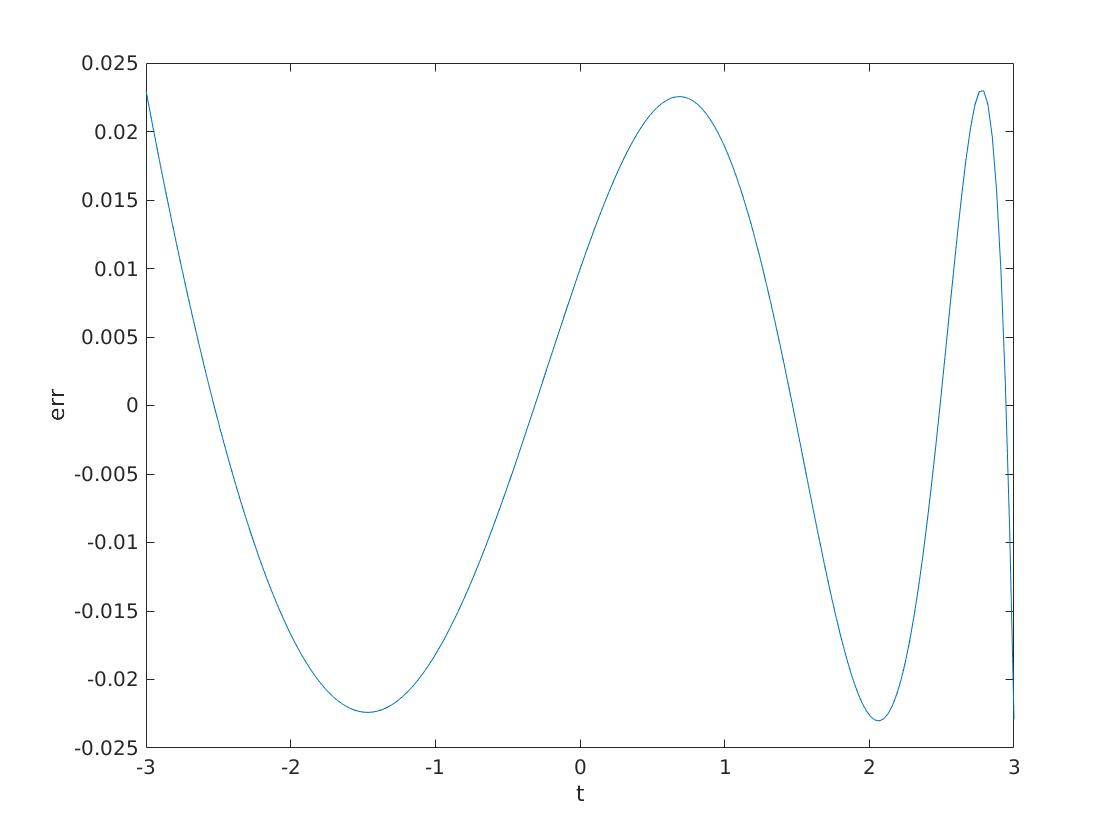
\includegraphics[scale=.30]{52_2.jpg}
\caption{Error for the given t value.}
\end{figure}

To solve we can use the bisection method:\\ 
\textbf{Code:}
\begin{lstlisting}
upper = exp(5);
lower = 0;
tolerance = .001
k = 201
t=(-3:6/(k-1):3)';
y=exp(t);
% 1 + t + t^2
T=[ones(k,1) t t.^2];

while upper - lower >= tolerance
    midpoint = (lower + upper)/2
    cvx_begin
    % a_0, a_1, a_2
    variable a(3)
    % b_0, b_1
    variable b(2)
    subject to
        abs(T*a-y.*(T*[1;b])) <= midpoint*T*[1;b]
    cvx_end
    if strcmp(cvx_status,'Solved')
        a_star = a;
        b_star = b;
        upper = midpoint;
        value = midpoint;
    else
        lower = midpoint       
    end
end

y_star = T*a_star./(T*[1;b_star]);
y_star
a_star
b_star

figure(1);
plot(t,y,'g', t,y_star,'r');
xlabel('t');
ylabel('y');

figure(2);
plot(t, y_star-y);
xlabel('t');
ylabel('err');
\end{lstlisting}
\textbf{Results:}\\
$a_star =\\
    1.0099\\
    0.6115\\
    0.1133\\
b\_star =\\
   -0.4147\\
    0.0485\\$
\subsection*{5.6}
Note: I do not deserve full credit for the below code. It was infered from the given code and solutions online.

\textbf{Code:}
\begin{lstlisting}
% tv_img_interp.m
% Total variation image interpolation.
% Defines m, n, Uorig, Known.
% Load original image.
pwd()
Uorig = double(imread('/home/carl/CUBoulder/coursework/5254/HW5/tv_img_interp.png'));
[m, n] = size(Uorig);
% Create 50% mask of known pixels.
rand('state', 1029);
Known = rand(m,n) > 0.5;
%%%%% Put your solution code here
% Calculate and define Ul2 and Utv.
% Placeholder:
cvx_begin
variable Ul2(m, n);
Ul2(Known) == Uorig(Known);
Ux = Ul2(2:end,2:end) - Ul2(2:end,1:end-1);
Uy = Ul2(2:end,2:end) - Ul2(1:end-1,2:end);
% Squared / l2 norm
minimize(norm([Ux(:); Uy(:)], 2)); 
cvx_end
cvx_begin
variable Utv(m, n);
Utv(Known) == Uorig(Known);
Ux = Utv(2:end,2:end) - Utv(2:end,1:end-1);
Uy = Utv(2:end,2:end) - Utv(1:end-1,2:end);
% abs or l1 norm
minimize(norm([Ux(:); Uy(:)], 1)); % tv roughness measure
cvx_end
%%%%%
% Graph everything.
figure(1); cla;
colormap gray;
subplot(221);
imagesc(Uorig)
title('Original image');
axis image;
subplot(222);
imagesc(Known.*Uorig + 256-150*Known);
title('Obscured image');
axis image;
subplot(223);
imagesc(Ul2);
title('l_2 reconstructed image');
axis image;
subplot(224);
imagesc(Utv);
title('Total variation reconstructed image');
axis image;
\end{lstlisting}
\textbf{Results:}\\
\begin{figure}[h]
\centering
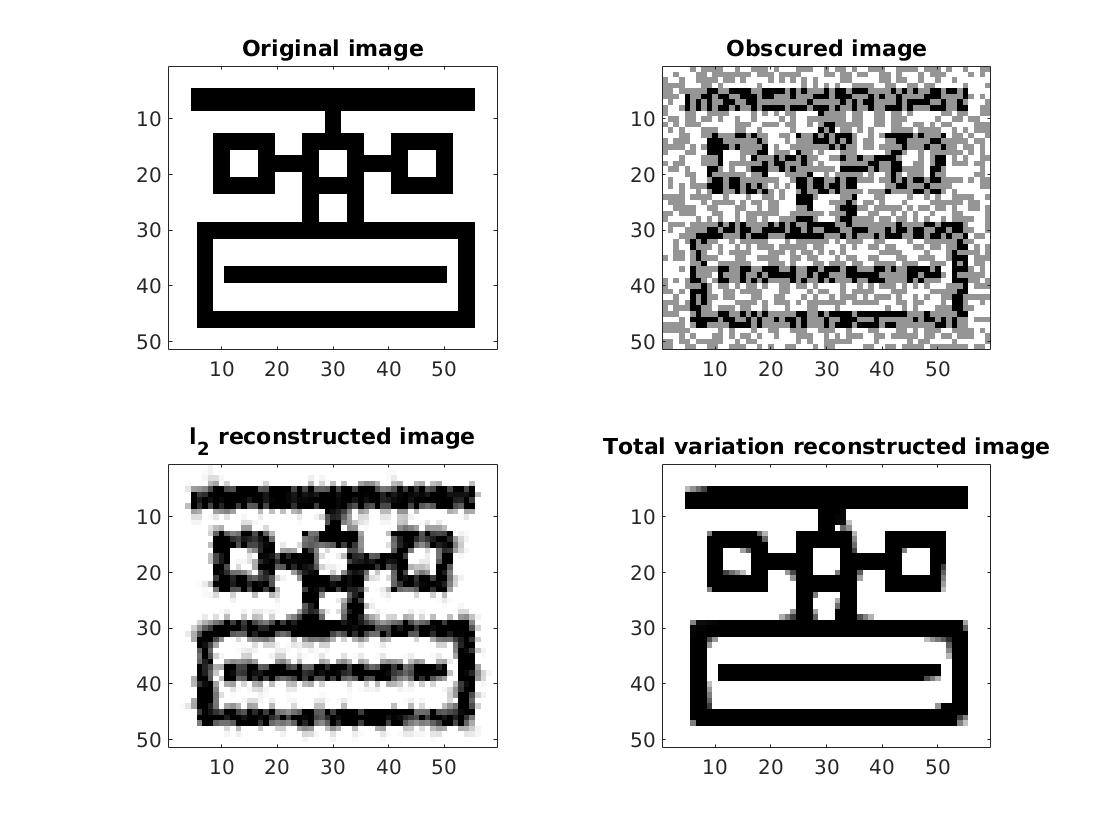
\includegraphics[scale=.30]{interpolation.jpg}
\caption{Interpolation results.}
\end{figure}

\subsection*{5.13}
\subsubsection*{a)}
We constrain the problem such that $c^Tx_i$ for all censored data points ($i=M+1,\dots,K$) must be greater than the lower bound $D$ while minimizing the uncensored data $i=1,\dots,M$.
\begin{equation*}
\begin{aligned}
& \underset{c}{\text{minimize}}
& & \sum_{i=1}^{M}(y_i-c^Tx_i)^2\\
& \text{subject to}\
& & c^Tx_i \ge D, \text{ for } i=M+1,\dots,K
\end{aligned}
\end{equation*}
\subsubsection*{b)}
\textbf{Code:}
\begin{lstlisting}
% data for censored fitting problem.
randn('state',0);
n = 20; % dimension of x's
M = 25; % number of non-censored data points
K = 100; % total number of points
c_true = randn(n,1);
X = randn(n,K);
y = X'*c_true + 0.1*(sqrt(n))*randn(K,1);
% Reorder measurements, then censor
[y, sort_ind] = sort(y);
sort_ind
X = X(:,sort_ind);
D = (y(M)+y(M+1))/2;
y = y(1:M);
X_uncen = X(:,1:M)
X_cen = X(:,M+1:K)
cvx_begin
    variable c(n)
    minimize(sum_square(y - X_uncen'*c))
    subject to
        X_cen'*c >= D
cvx_end
cvx_begin
    variable c_ls(n)
    minimize(sum_square(y - X_uncen'*c_ls))
cvx_end

norm(c - c_true, 2) / norm(c_true,2)

norm(c_ls - c_true, 2) / norm(c_true,2)
\end{lstlisting}
\textbf{Results:}\\
Errors:\\
$\hat{c} = 0.1538$\\
$c_{ls} = 0.3907$

\subsection*{5.15}
\subsubsection*{a)}
We can optimize the following:
\begin{equation*}
\begin{aligned}
& \underset{P}{\text{minimize}}
& & \frac{1}{N}\sum_{i=1}^{N}(d_i - (x_i-y_i)^TP(x_i-y_i))^2\\
& \text{subject to}\
& & P \succeq 0
\end{aligned}
\end{equation*}
Another approach would be to maxmize $i=1,\dots,M$ dissimilar points for the P-metric while keep $i=M+1,\dots,N$ similar points less then some arbitrarily small value $\alpha$:
\begin{equation*}
\begin{aligned}
& \underset{P}{\text{maxmize}}
& & \sum_{i=1}^{M}((x_i-y_i)^TP(x_i-y_i))^\frac{1}{2}\\
& \text{subject to}\
& & P \succeq 0\\
& & & \sum_{i=M+1}^{N}(x_i-y_i)^TP(x_i-y_i) \le \alpha
\end{aligned}
\end{equation*}
\subsubsection*{b)}
\textbf{Code:}
\begin{lstlisting}
%% data for learning a quadratic metric
% provides X, Y, d, X_test, Y_test, d_test
rand('seed',0);
randn('seed',0);
n = 5; % dimension
N = 100; % number of distance samples
N_test = 10;
X = randn(n,N);
Y = randn(n,N);
X_test = randn(n,N_test);
Y_test = randn(n,N_test);
P =randn(n,n);
P = P*P'+eye(n);
sqrtP = sqrtm(P);
d = norms(sqrtP*(X-Y)); % exact distances
d = pos(d+randn(1,N)); % add noise and make nonnegative
d_test = norms(sqrtP*(X_test-Y_test));
d_test = pos(d_test+randn(1,N_test));
P
alpha = 5;
[d_test, sort_ind] = sort(d_test);
X_test = X_test(:,sort_ind);
Y_test = Y_test(:,sort_ind);
diff = X_test-Y_test

clear P sqrtP;
cvx_begin
    variable P(n,n)
    minimize((1/N_test)*pow_pos(sum(d_test' - sqrt(diag(diff'*P*diff))),2)),
    subject to
    P>0
cvx_end

\end{lstlisting}
\textbf{Result:}
Mean Squared Error = +1.24901e-10

\subsection*{6.4}
\subsubsection*{a)}
Since the noise determans the stoachsticity, the cumulative distribution function for the normal distrubtion can be defined as follows:
$$\Phi(\frac{x-u}{\sigma})$$
where
$$x=y_i(a_{i,j}-a_{i,k})$$
This gives:
$$\Phi(\frac{y_i(a_i-a_j)}{\sigma})$$
Thus the total probability of outcomes y given abilities a is:
$$p(y|a)=\prod_{i=1}^{n}\Phi(\frac{y_i(a_i-a_j)}{\sigma})$$
The log likelihood is:
$$l(a) = \sum_{i}^{n}log(\Phi(\frac{y_i(a_i-a_j)}{\sigma}))$$
This is concave so we can minimie the negative log likelihood:
\begin{equation*}
\begin{aligned}
& \underset{a}{\text{minimize}}
& & \sum_{i}^{n}log(\Phi(\frac{y_i(a_i-a_j)}{\sigma}))\\
& \text{subject to}\
& & 0 \preceq a \preceq 1
\end{aligned}
\end{equation*}
The constraint is a relaxation of the binary constraint:
$$a_i \in {0,1}$$

\subsubsection*{b,c)}
\textbf{Code:}\\
\begin{lstlisting}
n = 10;
m = 45;
m_test = 45;
sigma= 0.250;
test = [...]
train = [...]

A1 = sparse(1:m,train(:,1),train(:,3),m,n);
A2 = sparse(1:m,train(:,2),-train(:,3),m,n);
A = A1+A2;

cvx_begin
    variable a_hat(n)
    minimize(-sum(log_normcdf(A*a_hat/sigma)))
    subject to
    a_hat >= 0
    a_hat <= 1
cvx_end
a_hat

res = sign(a_hat(test(:,1))-a_hat(test(:,2)));
Pml = 1-length(find(res-test(:,3)))/m_test
\end{lstlisting}
\textbf{Results b):}\\
$a\_hat =\\
    1.0000\\
    0.0000\\
    0.6829\\
    0.3696\\
    0.7946\\
    0.5779\\
    0.3795\\
    0.0895\\
    0.6736\\
    0.5779\\
$
\textbf{Results c):}\\
$P_{ml} = 0.8667$\\
About 86\% of the time time, the ML prediction is correct. 

\subsection*{6.6}
\subsubsection*{a)}
Our noise is I.I.D from a gaussian distribution we can minimize the sum of squares likelihood, expressing $v(t)$ in terms of the other components:
\begin{equation*}
\begin{aligned}
& \underset{x}{\text{minimize}}
& & \sum_{t=2}^{N+2}(y(t)-\sum_{\tau=1}^{k}h(\tau)x(t-\tau))^2\\
& \text{subject to}\
& & x(N) \ge x(N-1) \ge ... \ge x(1) \ge 0\\
& & & x(t) = 0, t \le 0
\end{aligned}
\end{equation*}
Since x monotonically increases with t, we can minimize.

\textbf{Code:}
\begin{lstlisting}
clear all; close all;
% create problem data
randn('state',0);
N = 100;
% create an increasing input signal
xtrue = zeros(N,1);
xtrue(1:40) = 0.1;
xtrue(50) = 2;
xtrue(70:80) = 0.15;
xtrue(80) = 1;
xtrue = cumsum(xtrue);
% pass the increasing input through a moving-average filter
% and add Gaussian noise
h = [1 -0.85 0.7 -0.3]; k = length(h);
yhat = conv(h,xtrue);
y = yhat(1:end-3) + randn(N,1);


cvx_begin
    variable x(N-1)
    minimize(pow_pos((y - conv(h,x)),2))
    subject to
        x >= 0
cvx_end
\end{lstlisting}
\textbf{Results:}\\
Cannot figure out how to express the above problem in CVX.

\subsection*{12.4}

We can formulate this as a SOCP for quasiconvex optimization.

Formulating the level set:
$$\set(S_{ij},t | \frac{\alpha p_j}{|||x_i-x_j||^2} \le t | S_{ij} \ge \beta R_{ij} )$$
\begin{equation*}
\begin{aligned}
& \underset{t}{\text{minimize}}
& & t\\
& \text{subject to}\
& &  t|||x_i-x_j||^2 \le -\alpha p_j \\
& & & \beta > 0, R_{ij} \ge 0
\end{aligned}
\end{equation*} 


\subsection*{15.3}
\subsubsection*{a)}
We want to maxmize the given logarithm network utility as it is a concave function.
\begin{equation*}
\begin{aligned}
& \underset{t}{\text{maxmize}}
& & \sum_{j=1}^{n}log(f_j)\\
& \text{subject to}\
& &  Rf \preceq c, f \succeq 0
\end{aligned}
\end{equation*} 

\subsubsection*{b)}
Latency is the sum of link delays when the link traffic $t_i$ is zero. $$d_i = \frac{1}{c_i}$$ resulting in zero flow. The link delay vector can be repesented as:

$$(\frac{1}{c_1},\dots,\frac{1}{c_m})$$
To some these delays, wil multply by $R^T$ and find the maximum element to get $L^{min}$:
$$L^{min}=max(R^T(\frac{1}{c_1},\dots,\frac{1}{c_m})$$
This imples that the minimum latency is the maximum of the flow latency.

\subsubsection*{c)}
We still want to maximize the logirthm network utility, however we can ensure that the latency is minimial, which can be expressed as an additional constraint:

\begin{equation*}
\begin{aligned}
& \underset{t}{\text{maxmize}}
& & \sum_{j=1}^{n}log(f_j)\\
& \text{subject to}\
& & Rf \preceq c, f \succeq 0\\
&&& \sum_{i=1}^{m}\frac{R_{ij}}{c_i-r_i^Tf} \le L, j=1,\dots,n 
\end{aligned}
\end{equation*} 
The new constraint $\sum_{i=1}^{m}\frac{R_{ij}}{c_i-r_i^Tf} \le L$ implies that The network flow from i to j devided by the delay cannot be greater than the minimized latency.

\subsubsection*{d)}
Note I do not deserve full credit for this. Heavily inspired from a solution online:\\\\ 
\textbf{Code:}
\begin{lstlisting}
% max utility
cvx_begin
    variable f(n)
    maximize geo_mean(f)
    R*f <= c
cvx_end
Umax=sum(log(f));

% min latency
Lmin = max(R'*(1./c));

N = 20;
ds = 1.10*Lmin*logspace(0,1,N);
Uopt = [];
for d = ds
    cvx_begin
        variable f(n)
        maximize geo_mean(f);
        R'*inv_pos(c-R*f) <= d*ones(n,1)
    cvx_end
    Uopt = [Uopt n*log(cvx_optval)];
end
semilogx(ds,Uopt,'k-',[Lmin,ds],[Umax,ones(1,N)*Umax],... 
'k--',[1,1]*Lmin,[Uopt(1),Umax],'k--')

xlabel('L'); ylabel('U');
\end{lstlisting}
\begin{figure}[h]
\centering
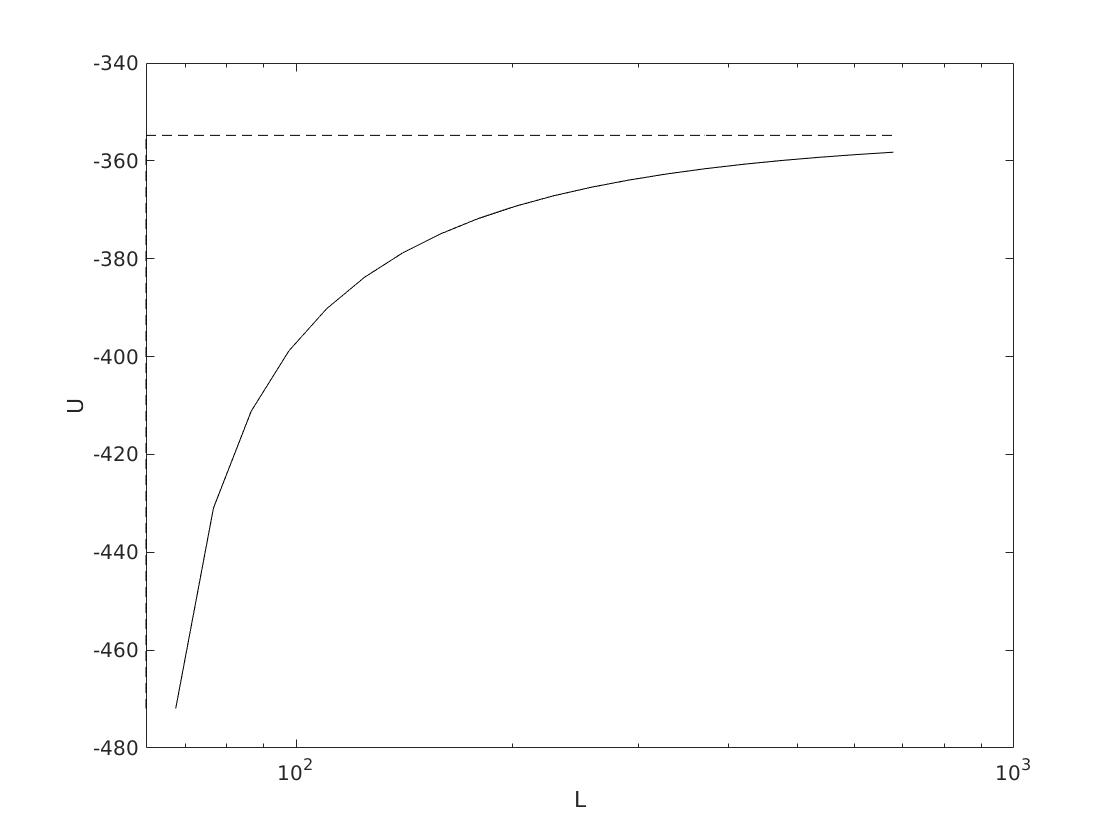
\includegraphics[scale=.2]{tradeoff.jpg}
\caption{Utilite vs latency tradeoff.}
\end{figure}


% --------------------------------------------------------------
%     You don't have to mess with anything below this line.
% --------------------------------------------------------------
 
\end{document}